\section{Tablas y figuras}

% Insertar una figura
\begin{figure}
  \centering
  \includegraphics[width=0.75\textwidth,clip=true]{\logoUniversidad}
  \caption{Logo de la Universidad.}
  \label{fig:logo_universidad}
\end{figure}


\begin{figure}
   \centering

  \begin{minipage}{0.45\textwidth}
   \centering

     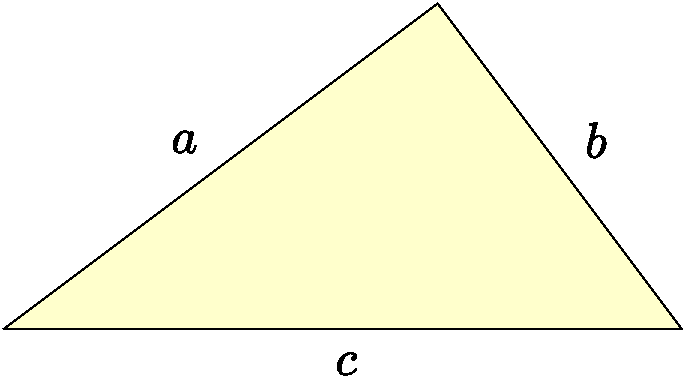
\includegraphics[clip=true,width=\textwidth]{triangulo_grande_bb.pdf}\\

    \footnotesize (a)
  \end{minipage}
  \hfill
  \begin{minipage}{0.45\textwidth}
   \centering
     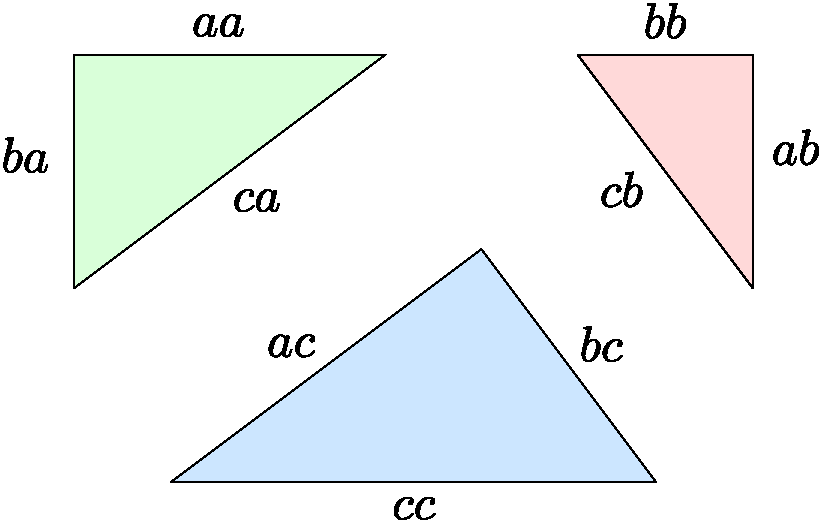
\includegraphics[clip=true,width=\textwidth]{triangulos_separados_bb.pdf}\\

   \footnotesize (b)
  \end{minipage}

    \bigskip

    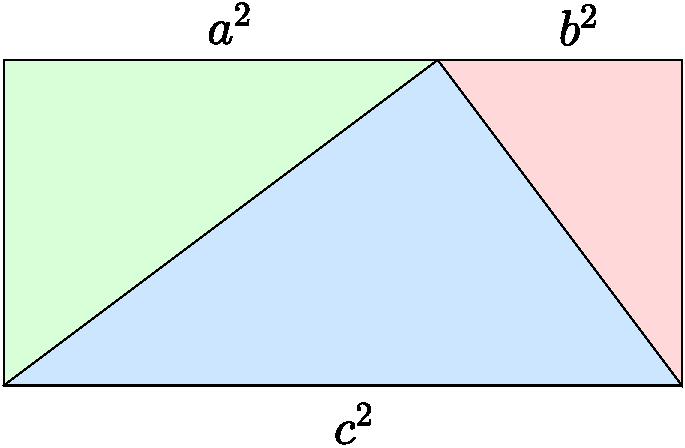
\includegraphics[clip=true,width=0.5\textwidth]{triangulos_unidos_bb.pdf}\\
    \footnotesize (c)

  \caption{Ejemplo con varias figuras. Demostración visual del teorema de Pitágoras. En (a) tenemos un triángulo rectángulo con hipotenusa $c$ y catetos $a$ y $b$. En (b) se muestra tres copias escaladas del mismo triángulo. El verde se ha escalado por $a$, el rojo/rosa por $b$, y el azul por $c$. En (c) se juntan los triángulos de (b) para formar un rectángulo cuya base es $c^{2}$, pero también $a^{2} + b^{2}$. Por tanto, $a^{2} + b^{2} = c^{2}$.}\label{fig:teoremapitagoras}
\end{figure}

\newpage
% También con \pagebreak